\section{Dissertation outline}
\label{chap1:sec2}




 The main contributions of the dissertation are divided into four articles/chapters, each focusing on defining and answering different aspects of pedestrian related challenges of the future urban networks. An overview of the dissertation is shown in \cref{fig: framework}.


\cref{chap1b} presents a background on the fundamentals of pedestrian research studies, including data collection methods, behavioural modelling, and novel methodologies in the field.
This chapter discusses the recent developments and techniques in pedestrian crossing behaviour and and how modern data-driven modelling is changing the traditional approaches of pedestrian studies. The proposed methods in this dissertation based on these data-driven approaches enable the use of deep learning algorithms to study behaviours of pedestrians more accurately.
This chapter also addresses the drawbacks and disadvantages of current modelling methods, and discusses the importance of interpretation in machine learning-based models.


\cref{chap2} introduces a semi-supervised deep modelling framework to utilize passively collected Wi-Fi data and detect the transportation mode of network users in a congested urban area. Using Wi-Fi data as an alternative source of data provides the opportunity to exploit large scale, passively collected and pervasive data in pedestrian studies. In addition, semi-supervised nature of the model helps incorporate low-cost unlabelled data in large scales. By developing an advanced residual network, we can distinguish network users, including pedestrians in highly congested urban areas of downtown Toronto using their WiFi signal patterns.

\cref{chap3} is dedicated to investigation of Virtual Reality (VR) data, as another state of the art source of data gaining significant improvements and popularity in recent years. Using VR for data collection enables exploring pedestrian behaviour in hypothetical scenarios which might be dangerous to investigate otherwise. By developing a VR version of a crossroad, participants are asked to cross a simulated street under different conditions, and while distracted by their smartphones in some scenarios. To analyze crossing behaviour of pedestrians and assess the effect of smartphone distraction, a survival analysis is developed.

The next two chapters investigate the interactions of Automated Vehicles (AV) and pedestrians. As automated vehicles are going to find their ways on streets in near future, they will have a significant impact on dynamics of urban areas. This phase of the research aims to quantify the effects of specific AV traffic parameters and features of future streets on pedestrians' walking behaviour.

\cref{chap4} is an extensive analysis of pedestrian road crossing behaviour, in the presence of automated vehicles. Followed by a large and efficiently designed data collection campaign using virtual reality, data-driven neural network-based survival models are developed to understand the changes that are expected to occur in the future of urban roads. Furthermore, interpretability of the neural networks of widely discussed, and a game theory based post-hoc method is implemented to explain the output of the model. Finally, a discussion on the results, their policy implications for future decision making in the cities, and suggestions on running data collection experiments using VR conclude this chapter.

\cref{chap6} presents another aspect of pedestrian crossing behaviour confronting automated vehicles. Using the same dataset as in \cref{chap4}, trajectory of pedestrians is modelled using data-driven time-series modelling. This chapter also includes an extensive review of open-access video data of real automated vehicles provided by some of the AV manufacturers, and drawbacks and advantages of each of the datasets. VR data enables studying specific behaviours of pedestrians under customized conditions, and therefore they are shown to be an important alternative to real datasets for various purposes. Advanced machine learning models are trained to predict the trajectory of pedestrians considering their initial trajectory, head orientations and distance to vehicles, as well as other environmental and contextual variables that can be captured by a typical automated vehicle. 

\cref{chap7} summarizes the findings from the previous four chapters and the limitations of the developed frameworks, datasets and methodologies.
Finally, it provides new research questions for future work and possible extensions to pedestrian behaviour analysis.



 \begin{figure}
   \centering
   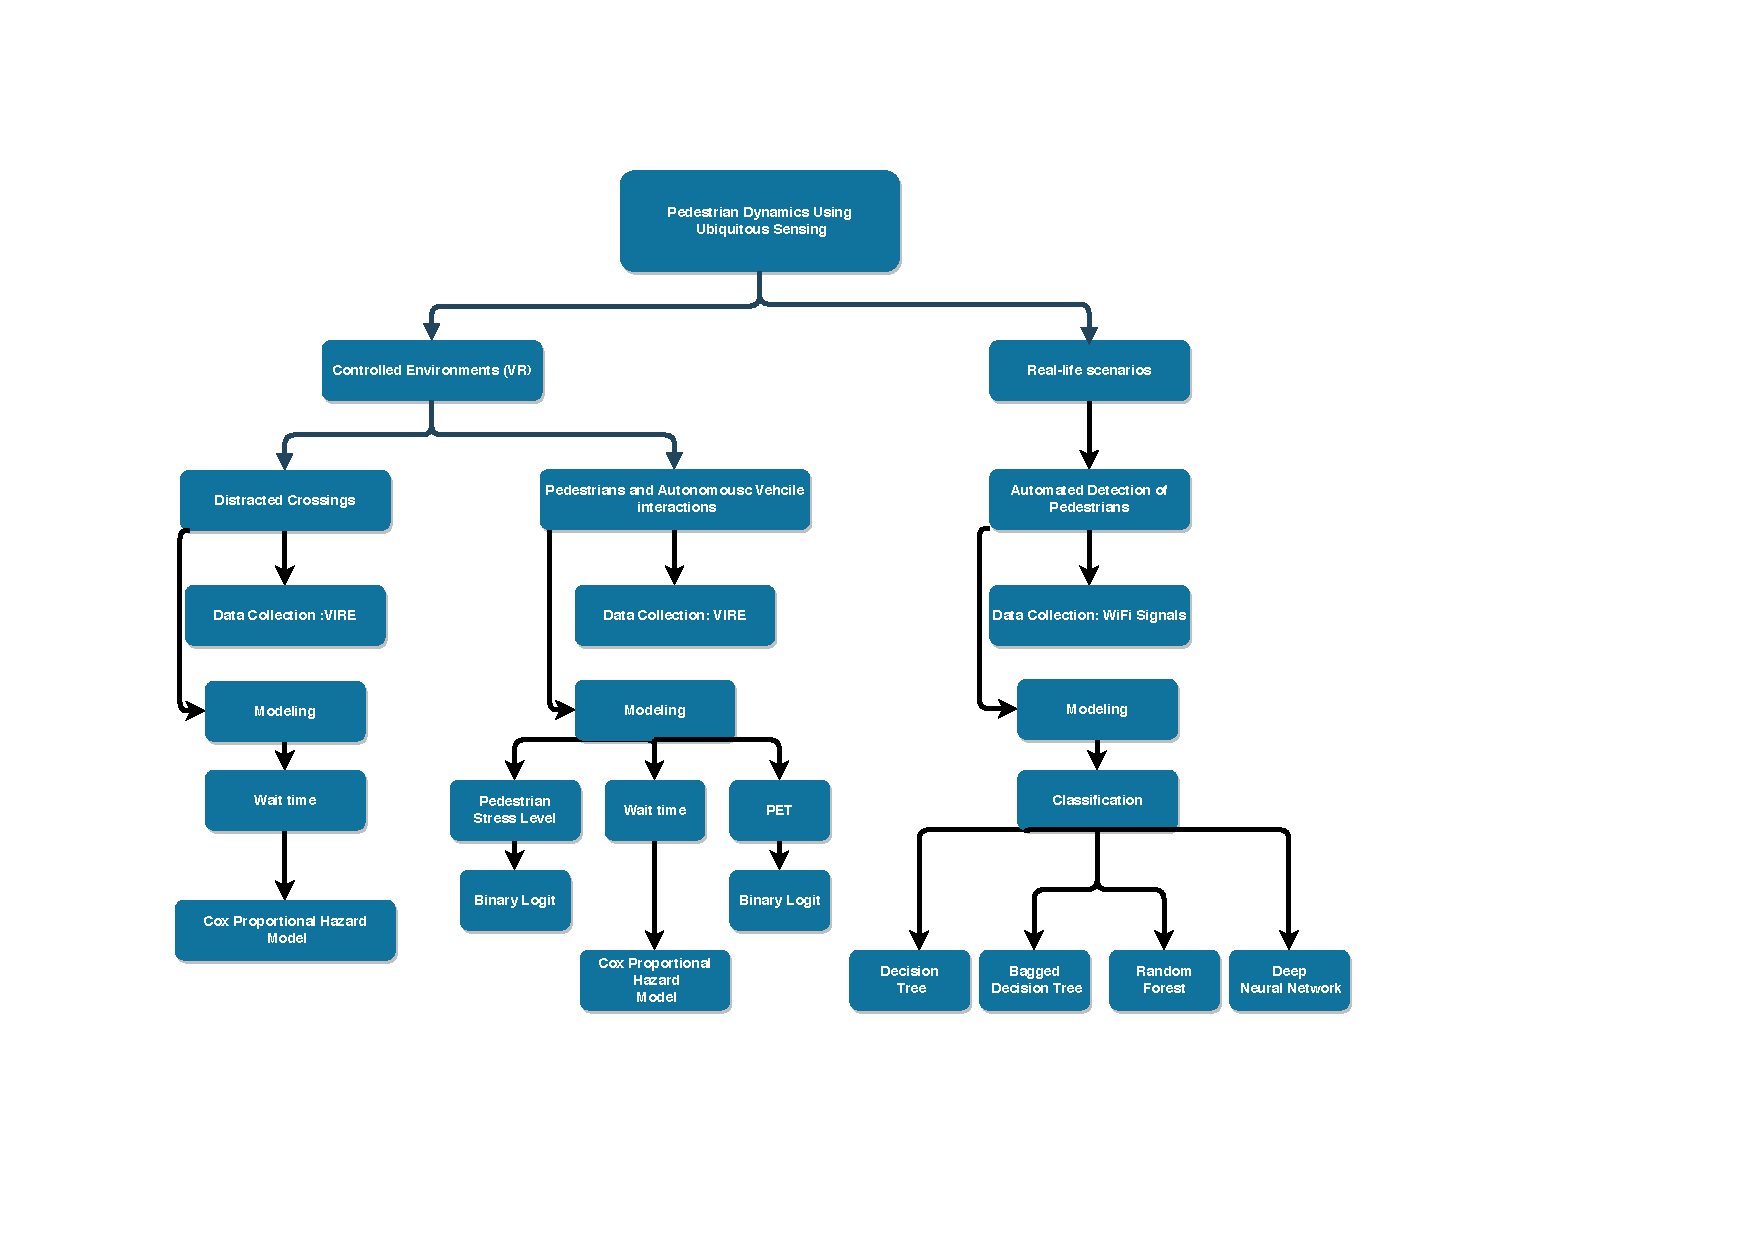
\includegraphics[width=\textwidth]{chapter_1/figures/frame.pdf} % trim=left bottom right top
   \caption{Dissertation Overview}
   \label{fig: framework}
 \end{figure}